% For instructions,
\documentclass[reprint, amsmath, amssymb, aps]{revtex4-2}

%\usepackage[norsk]{babel}
%Uncomment this if you want to write in Norwegian

\usepackage{graphicx}% Include figure files
\usepackage{dcolumn}% Align table columns on decimal point
\usepackage{bm}% bold math
\usepackage{hyperref}% add hypertext capabilities
\usepackage{booktabs}
\usepackage{float}



\begin{document}
\title{Project1 - FYS4460}
\author{Mikkel Metzsch Jensen}

\date{\today}
\maketitle

\subsection*{a) Maxwell Boltzman distribution}
We simulate a $15 \times 15 \times 15$ Lennard Jones system with face-centered-cubic packing resulting in 13500 particles. We use temperature $T' = 2.5 \ \epsilon/k_B$  and simulate for 30000 timesteps with default timestep length $0.005 \tau$. See script \textit{a.in} for more details. We then looked at the velocity distribution for the last timestep in form of a histogram shown in figure \ref{fig:hist_dist}.
\begin{figure}[H]
  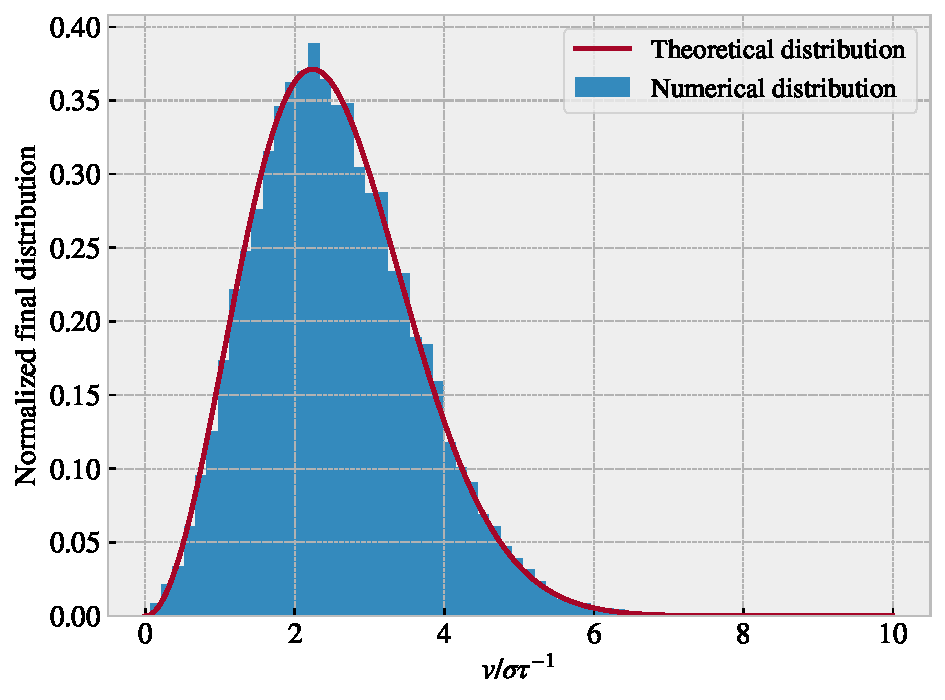
\includegraphics[width=\linewidth]{figures/MB_dist.pdf}
  \caption{Velocity distribution histogram for the final time-step $t_n$ in the simulation. The numerical results for the simulation matches nicely with the theoretically Maxwell-Boltzman distribution given as $f(v) = \left(\frac{m}{2\pi kT}\right)^{3/2}4\pi v^2e^{-\frac{mv^2}{2kT}}$.}
  \label{fig:hist_dist}
\end{figure}
We see that the final velocity distribution found in the simulation matches quite well with the theoretical Maxwell-Boltzmann distribution. In order to examinate how fast this distribution is reached we calculate the inner product given as:
\begin{align}
  \frac{\sum_i h_i(t)h_i(t_n)}{\sum_i h_i(t_n)^2}
  \label{eq:inner_product}
\end{align}
where $h_i$ is the height of bin $i$ in the histogram and $t_n$ is the final time-step. By calculating \ref{eq:inner_product} as a function of time we get the result shown in figure \ref{fig:inner_product}. As a quick estimate we can say that the distribution is reached after approximately $30 \tau$ when the inner product has roughly converted to 1. Since the inner product stays around 1 we can conclude that the distirbution shown in \ref{fig:hist_dist} is indeed the steady state of this system.
\begin{figure}[H]
  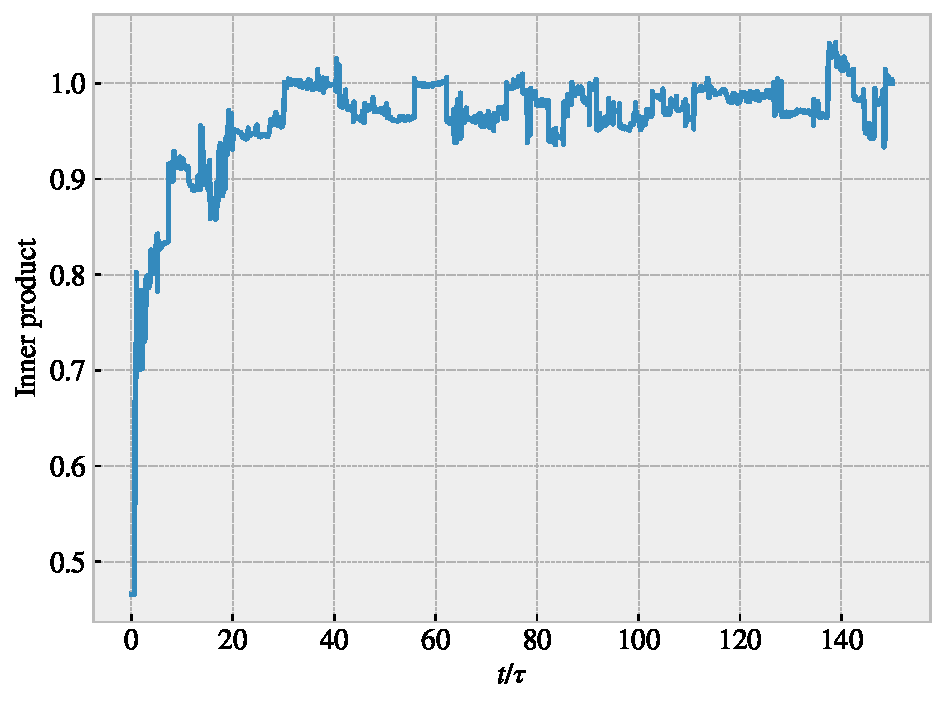
\includegraphics[width=\linewidth]{figures/inner_product.pdf}
  \caption{Inner product as shown in equation \ref{eq:inner_product}. We see that it converges towards approximately 1 indicating that it have reached the distirbution from \ref{fig:hist_dist}.}
  \label{fig:inner_product}
\end{figure}
%
%%
%
\subsection*{b) Total energy}
We use similar simulation settings as in a) (see script \textit{b.in}), where we now output the total energy with the fix ave/time command. We look at the development of the total energy over time for different timesteps as showed in figure \ref{fig:etotal}.
\begin{figure}[H]
  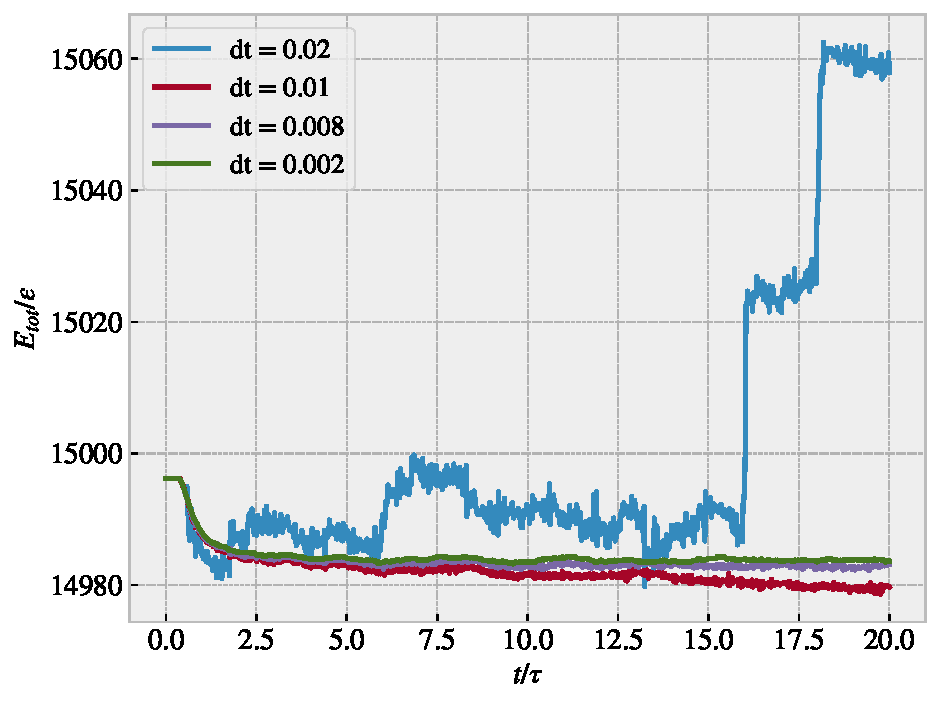
\includegraphics[width=\linewidth]{figures/Etot.pdf}
  \caption{Total energy over time for different timesteps $dt$.}
  \label{fig:etotal}
\end{figure}
We see as expected that the energy fluctuations is qualitatively bigger for bigger $dt$. We also notice that energy drops over the first period of the simulation. This is probably due to the system stabilization taken place. I'm not comepletly sure why this happens at NVE, where I would expect the energy to remain constant and instead having temperature fluctuations.

%
%%
%
\subsection*{c) Temperature}
We now consider the temperature in the simulation. We reuse the settings from script \textit{b.in} in the modified version in script \textit{c.in}. We use the equipartition principle:
\begin{align}
  \langle E_k \rangle = \frac{3}{2}Nk_bT
  \label{eq:equip}
\end{align}
where $E_k$ is the kinetic energy, $N$ the number of particles, $k_b$ Boltzmann's constant and $T$ is the temperature. By using this relation we find the temperature in the simulations for different $dt$. The result is showed in figure \ref{fig:temp}
\begin{figure}[H]
  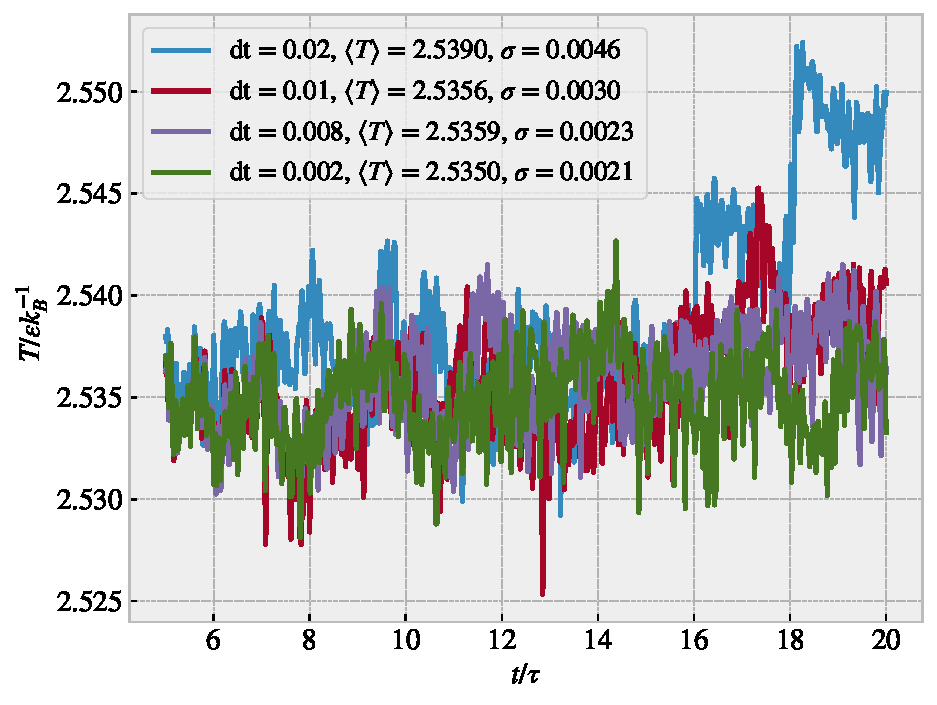
\includegraphics[width=\linewidth]{figures/temp.pdf}
  \caption{Estimated temperature using equation \ref{eq:equip} over time for different timesteps $dt$. Notice that the first period of time is excluded due to the equilibriation of the system.}
  \label{fig:temp}
\end{figure}
We initialized the simulations with temperature $T = 2.5$ which corresponds quite good to the mean value found here. All though we see a general ofsett of $\approx 0.035$ comparied to the initialized value of 2.5. This is due to the way that LAMMPS set the initial velocity distribution in order to reach the target temperature. In this process it does not take the potentiel energy into account which depends on the distance between the atoms at the initial state. When the simulaiton starts, the energy distribution with respect to kinetic and potentiel energy is redistributed such that it might not hit the target value exactly. The size and direction of the offset will therefore vary for different packing style and density. \par
By looking at the standard deviation $\sigma$, we see that the fluctuations is generally lower with decreasing $dt$. In order to see how the fluctuations depends on the system size we also ran a series of simulations with fixed $dt = 0.002$ but with increasing system size. This is shown in figure \ref{fig:temp_size}
\begin{figure}[H]
  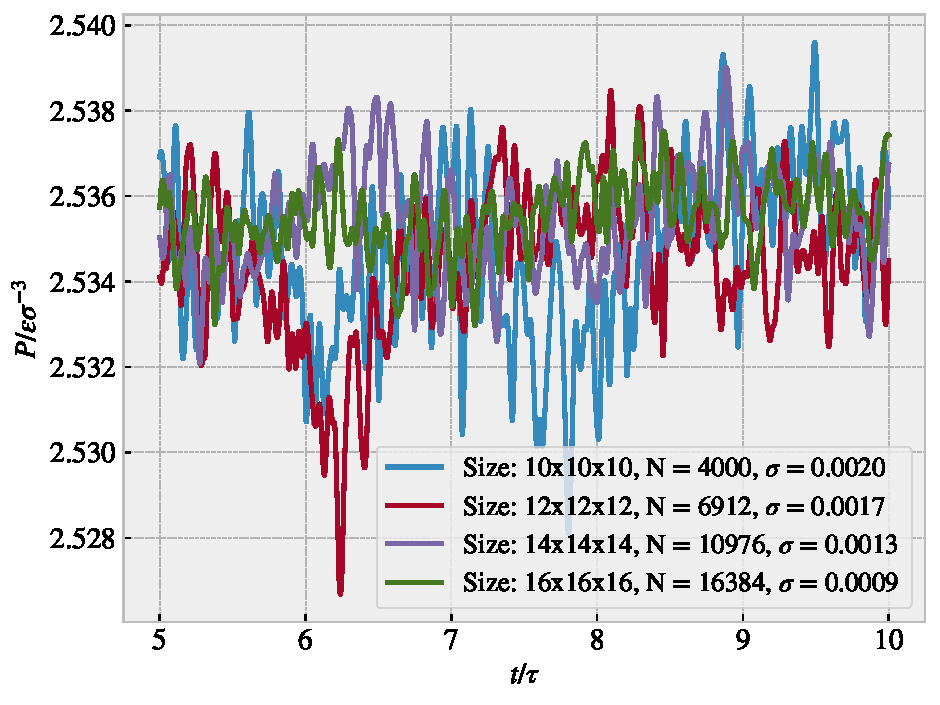
\includegraphics[width=\linewidth]{figures/temp_size.pdf}
  \caption{Estimated temperature using equation \ref{eq:equip} over time for different system sizes $a\times b\times c$ measured in number of unit cells. Each unit cell contains 4 atoms, which gives a total of $N = 4abc$ atoms.}
  \label{fig:temp_size}
\end{figure}
We see that the fluctuations generally gets smaller for bigger systems.
%
%%
%
\subsection*{d) Pressure as function of temperature}
We now perform a series of simulations at different temperature, let it stabilize, and then collect the average values for the pressure $P(T)$ as a function of average temperature $T$. See script \textit{d.in} and \textit{d.py} for more info. By plotting the pressure $P(T)$ with a linear fit we get the result showed in figure \ref{fig:P(T)}
\begin{figure}[H]
  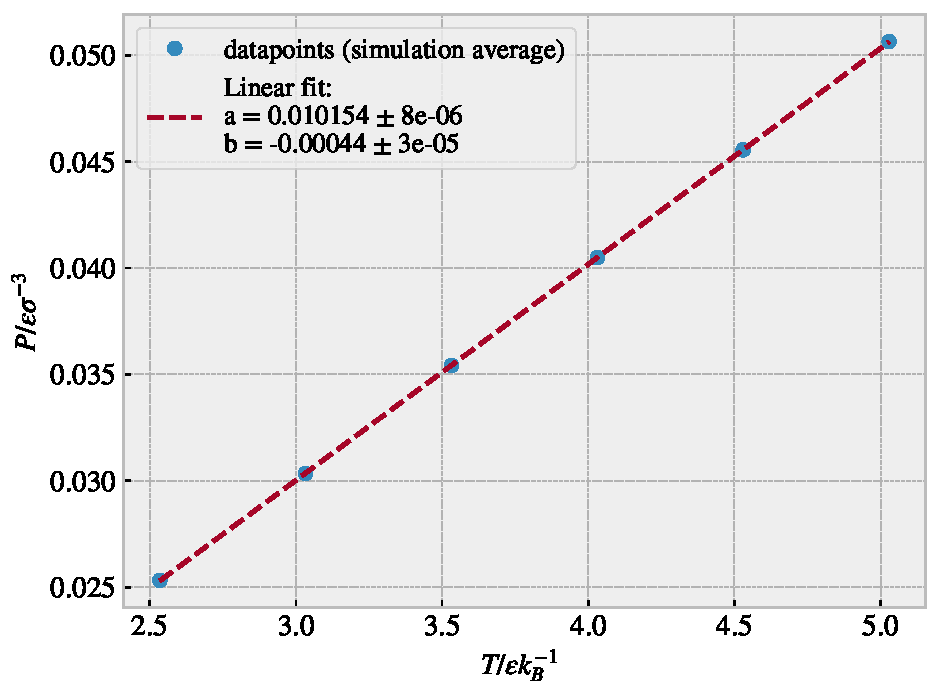
\includegraphics[width=\linewidth]{figures/P(T).pdf}
  \caption{Average measurements of temperature and pressure in stabilized simulations. The linear fit confirms the proportionality between pressure and temperature.}
  \label{fig:P(T)}
\end{figure}
We see that the result fit nicely to a linear model which is consistent with both the ideal gas law and also the Van der Waals equation which we will adress in the next exercise.
%
%%
%
\subsection*{e) Pressure as function of both temperature and density}
We now measure the pressure as a function of both temperature and density. We make a grid of values with 10 temperature points in the interval $T \in [1, 10]$ and 10 density points $\rho \in [0.02, 0.38]$ and simulate 100 times according to all the possible combination of theese values. See script \textit{e.in} and \textit{e.py} for more info. We then consider two models to predict the relationship between pressure, temperature and density. The first model is ideal gas law:
\begin{align*}
  PV = Nk_BT
\end{align*}
Since we have $k_B = 1$ in our simulations this model predicts a good linear fit between $PV$ adn $T$ with a slope of $N$. The second model to consider (which should be the one in use here) is the Van der Waals equation:
\begin{align*}
  (P + a \frac{N^2}{V^2})(V-Nb) = NkT
\end{align*}
From this we expect to see a linear fit bewteen  $(P + a \frac{N^2}{V^2})(V-Nb)$ and $T$ with slope $N$. \par
With the data from the simulations we try to fit the data to both of these models by performing linear regression with a fixed slope of $N$. For the Van der Wall model we use a python script to choose parameters $a$ adn $b$ such that the $MSE$ of the fits gets minimized. See script \textit{e.py} for more details. The results are shown in figure \ref{fig:TRP_ideal} and \ref{fig:TRP_waal}.

\begin{figure}[H]
  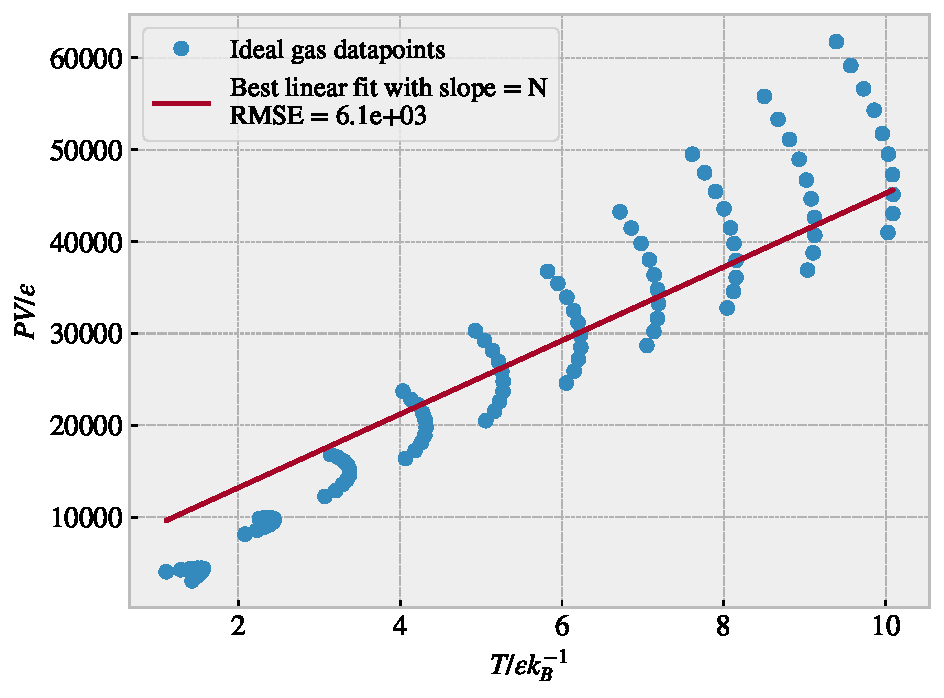
\includegraphics[width=\linewidth]{figures/TRP_ideal.pdf}
  \caption{Linear fit for ideal gas relation.}
  \label{fig:TRP_ideal}
\end{figure}

\begin{figure}[H]
  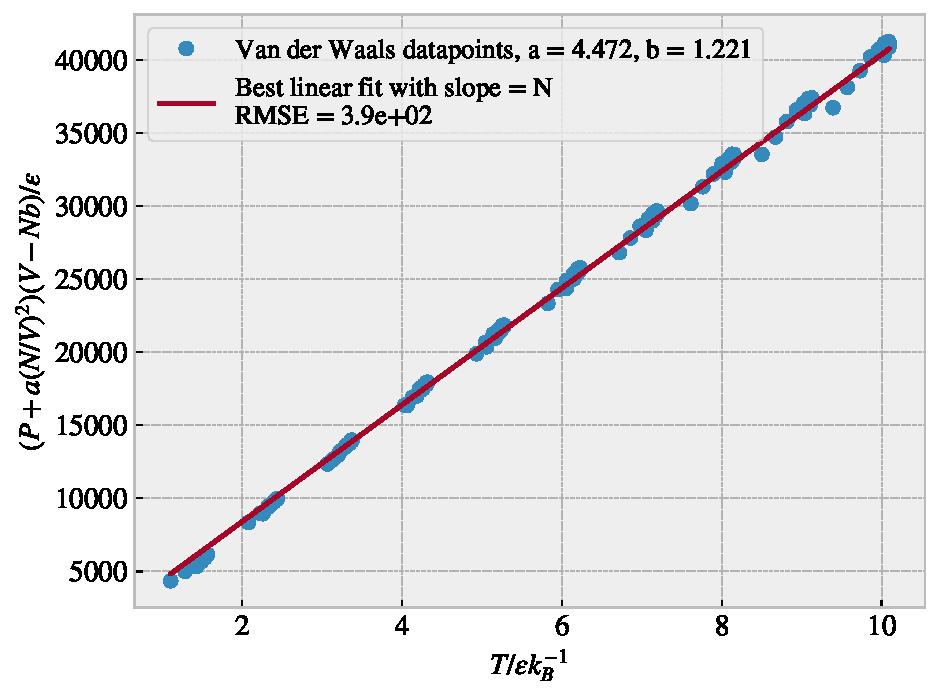
\includegraphics[width=\linewidth]{figures/TRP_waal.pdf}
  \caption{Linear fit for Van der Wall relation.}
  \label{fig:TRP_waal}
\end{figure}

We see that the van der waal fit is clearly the better one here, and we estimate the parameters to be $a = 4.472$ and $b = 1.221$
%
%%
%
\subsection*{f) Diffusion - mean square displacement}
We now look at the diffusion in the liquid phase of the Argon model. We measure the mean square displacement $\langle r^2(t) \rangle$ as a function of time for different temperatures. We use density $\rho = 0.8$ and temperatures $T = 0.9, 1.0, 1.1, 1.2$. See script \textit{f.in} and \textit{f.py} for more info. The result are shown in figure \ref{fig:msd}. By finding the slope $\langle r^2(t) \rangle / t$ we can estimate the diffusion constant though the theoretical relation:
\begin{align}
  \langle r^2(t) = 6Dt\rangle, \quad when \ t \rightarrow \infty
  \label{eq:diffusion}
\end{align}
\begin{figure}[H]
  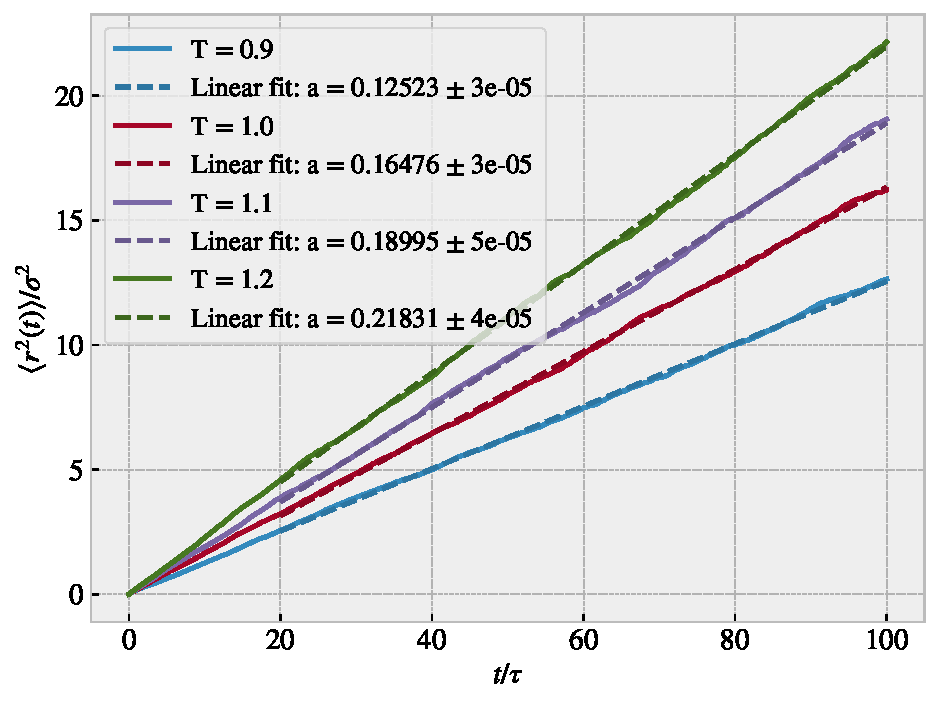
\includegraphics[width=\linewidth]{figures/diffusion.pdf}
  \caption{Measure of the mean square displacement $\langle r^2(t) \rangle $ as a function of time $t$ for different temperatures $T$ in the liquid phase of the Argon model. For this we used density $\rho$ = 0.8. The slope estimates the diffusion constant $D$ as $6D$ according to equation \ref{eq:diffusion}}
  \label{fig:msd}
\end{figure}
The diffusion constants estimated from figure \ref{fig:msd} is listed in table \ref{tab:D}
\begin{table}[H]
  \begin{center}
  \caption{Estimated diffusion constants from figure \ref{fig:msd}}
  \begin{tabular}{|c|c|} \hline
  \textbf{Temperature} [$T/\epsilon k_B^{-1}$] & \textbf{Diffusion constant} [$\sigma^2/\tau$]  \\ \hline
  0.9 & 0.02087 $\pm$ \num{3e-5} \\ \hline
  1.0 & 0.02746 $\pm$ \num{3e-5} \\ \hline
  1.1 & 0.03166 $\pm$ \num{5e-5} \\ \hline
  1.2 & 0.03638 $\pm$ \num{4e-5} \\ \hline
  \end{tabular}
  \label{tab:D}
  \end{center}
\end{table}
We then plot the diffusion constant as a function of temperature as shown in figure \ref{fig:diffusion_relation}.
\begin{figure}[H]
  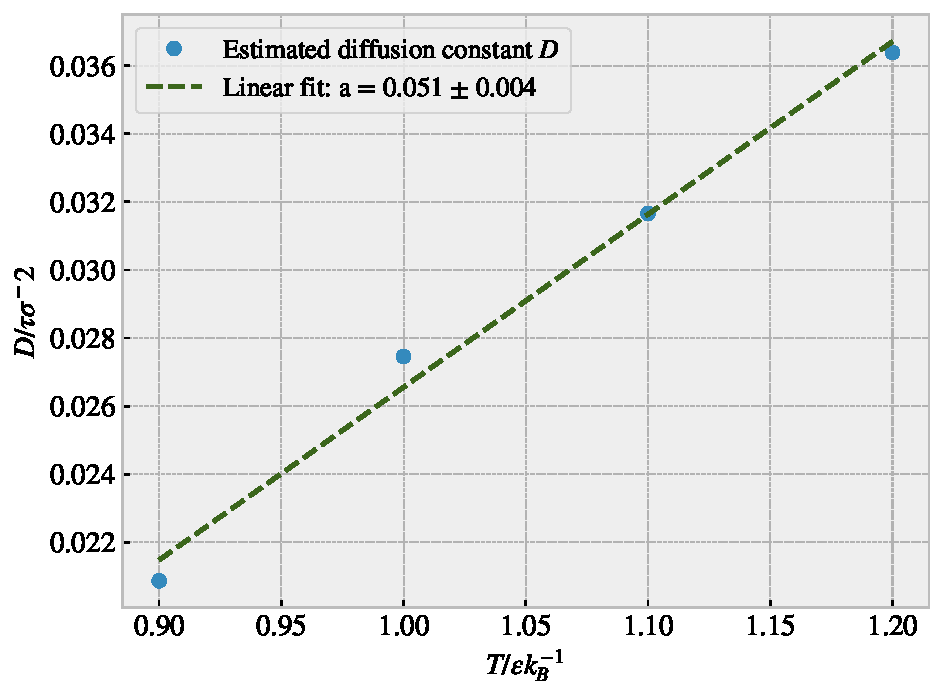
\includegraphics[width=\linewidth]{figures/diffusion_relation.pdf}
  \caption{The diffusion constant values from table \ref{tab:D} plotted against the temperature used.}
  \label{fig:diffusion_relation}
\end{figure}

From these datapoints it appears that the diffusion constant is proportional to the temperature with proportionality constant $a = 0.051 \pm 0.004$. This can be related to the Stokes-Einstein equation:
\begin{align*}
  D(t) = \frac{kT}{6\pi \mu r}
\end{align*}
where $\mu$ is the solvent viscosity, and $r$ is the radius of the diffusing particle. \\
\\
Another thing to notice is the behaviour of the mean square displacement measurements during the first few timesteps, which is highlighted in figure \ref{fig:diffusion_start}.

\begin{figure}[H]
  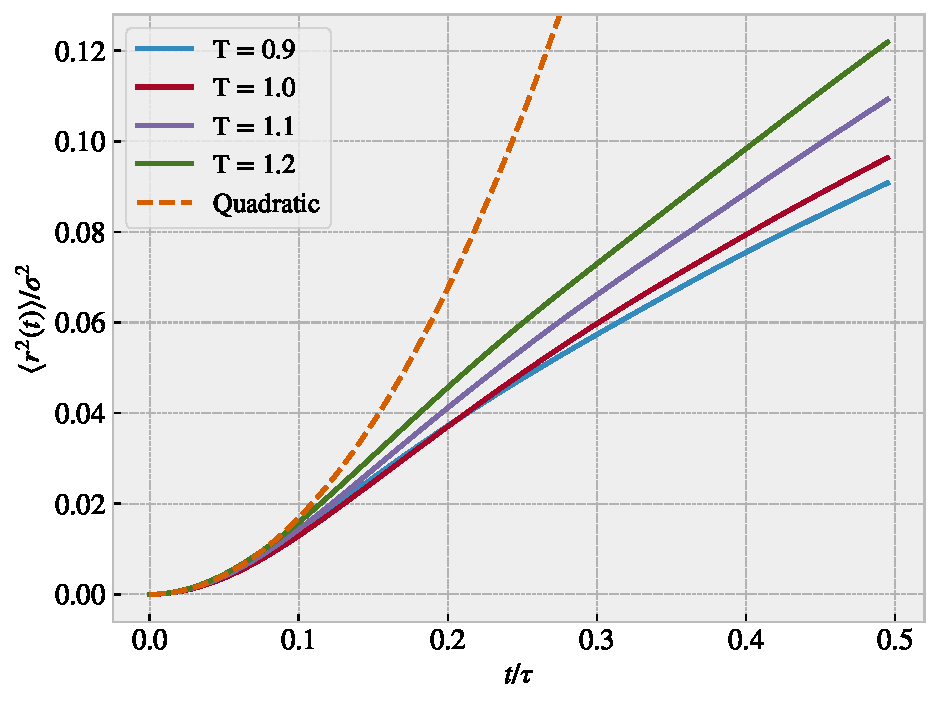
\includegraphics[width=\linewidth]{figures/diffusion_start.pdf}
  \caption{A zoom on the beginning of figure \ref{fig:msd} which shows a quadratic development before going into the linear relation as discussed.}
  \label{fig:diffusion_start}
\end{figure}
The quadratic development of MSD can be explained by the fact that the atoms move as $\vec{r}(t) = \vec{v}_0t + \vec{r}_0$ when far away from other atoms. In the beginning of the displacement measurements the atoms travel uninterupted for a short period of time and therefore the displacement goes as $r^2 \propto v_0^2t^2$. This is well showcased in the beginning of figure \ref{fig:diffusion_start}.
%
%%
%
\subsection*{g) Radial distribution function (rdf)}
We simulate two system corresponding to a argon in liquid phase and solid phase respectively. In both cases we let the system stabilize for 10000 timesteps and then compute the rdf as an average over another 10000 steps. Here we used $dt = 0.005$ and $T = 1.0$. For the liquid phase we used $\rho = 0.8$ and for the solid phase we used $\rho = 1.2$. We then compute the radial distribution function $g(r)$ in LAMMPS. See script \textit{g.in} and \textit{g.py} for more info. The results are showed in figure \ref{fig:rdf}

\begin{figure}[H]
  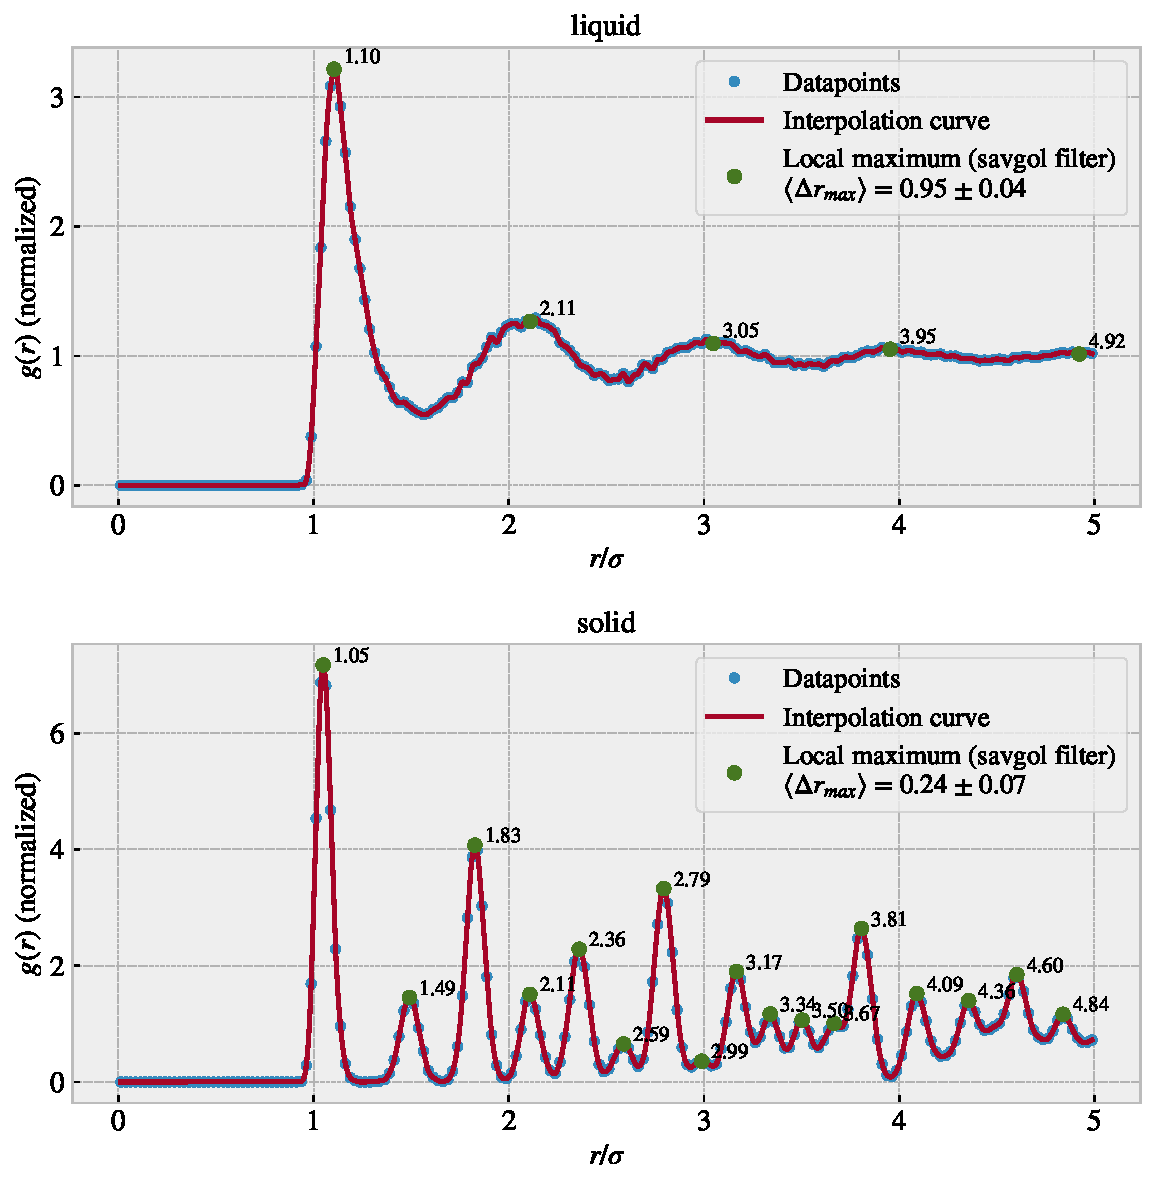
\includegraphics[width=\linewidth]{figures/rdf.pdf}
  \caption{Radial distirbution for argon in liquid ($\rho = 0.8$) and solid ($\rho = 1.2$) phase. We used a temperature of $T = 1.0$ in both simulation and calculate the average distirbution over 10000 timesteps with $dt = 0.005$ after stabilization for 10000 timesteps first.}
  \label{fig:rdf}
\end{figure}

As indicated on the plot we get distinct peaks in the radial distribution at certain distances. We see that the peaks are more sharp and narrow for the solid phase than the liquid. This makes perfectly sense since the atoms in the solid organizes itself in a crystal lattice to a greater extent than the liquid. If we take the average difference between theese peaks (not including the distance from the main atom to the first peak) we get the averages shown in the figure which is as follows:
\begin{align*}
  \langle \Delta r_{max} \rangle_{liquid} &= 0.95 \\
  \langle \Delta r_{max} \rangle_{solid} &= 0.24
\end{align*}
From this we see that the atoms in the solid are packed more closely together, as expected when comparing the solid and liquid phase of argon.
%
%%
%
\subsection*{j) Identifying differences and similarities between Stillinger-weber and Lennard Jones potential}
We look at the two-particle part of the Stillinger-Weber potentiel $V_2$. When ignorning the cut-off function we see that this is almost on the same form as the lennard jones potential $U(r)$:
\begin{align*}
  &V_2(r_{ij})_{(\text{no cut-off})}& &=& &A_{ij}\epsilon_{ij}\left[ B_{ij}\left(\frac{\sigma_{ij}}{r_{ij}}\right)^{p_{ij}} - \left(\frac{\sigma_{ij}}{r_{ij}}\right)^{q_{ij}} \right]& \\
  &U(r)& &=& &4\epsilon \left[\left(\frac{\sigma}{r}\right)^{12} - \left(\frac{\sigma}{r}\right)^{6}\right]&
\end{align*}
From the lennard jones potential we have the coresponding Stillinger-Weber parameters $A_{ij} = 4$, $B_{ij} = 1$, $p_{ij} = 12$, $q_{ij} = 6$. From the Si.sw file we read that theese parameters are set to
\begin{align*}
  &A = 7.049556277& &B = 0.6022245584& &p = 4.0& &q = 0.0&
\end{align*}
Here we see the most significant difference in $p$ and $q$ which determines the strength of the the pauli repulsion ($p$) and coloumb attraction ($q$) respectively. Thus we have a minimal strength of the coloumb attraction and also a heavily reduced strength of the pauli repulsion, which is further reduced by $B < 1$. The difference in $A$ is not really significant.
%
%%
%
\subsection*{k) Simulating three states of Si with Stillinger-Weber potential }
We now want to visualize the simulations of the Si system in solid, liquid and gas states. By a quick look on wikipeadia: \url{https://en.wikipedia.org/wiki/Silicon} we find that the melting point of silicon is $T_{\text{melting}} = 1687$ K and the boiling point is $T_{\text{boiling}} = 3538$ K. We therefore run the simulations on temperatures: 400 K, 3000 K and 8000 K to achieve a simmulaiton at solid, liquid and gas states respectively. See script \textit{k.in} for more info. We visualize the final frame of our simulations in ovito shown in figure \ref{fig:3_states}.
\begin{figure}[H]
  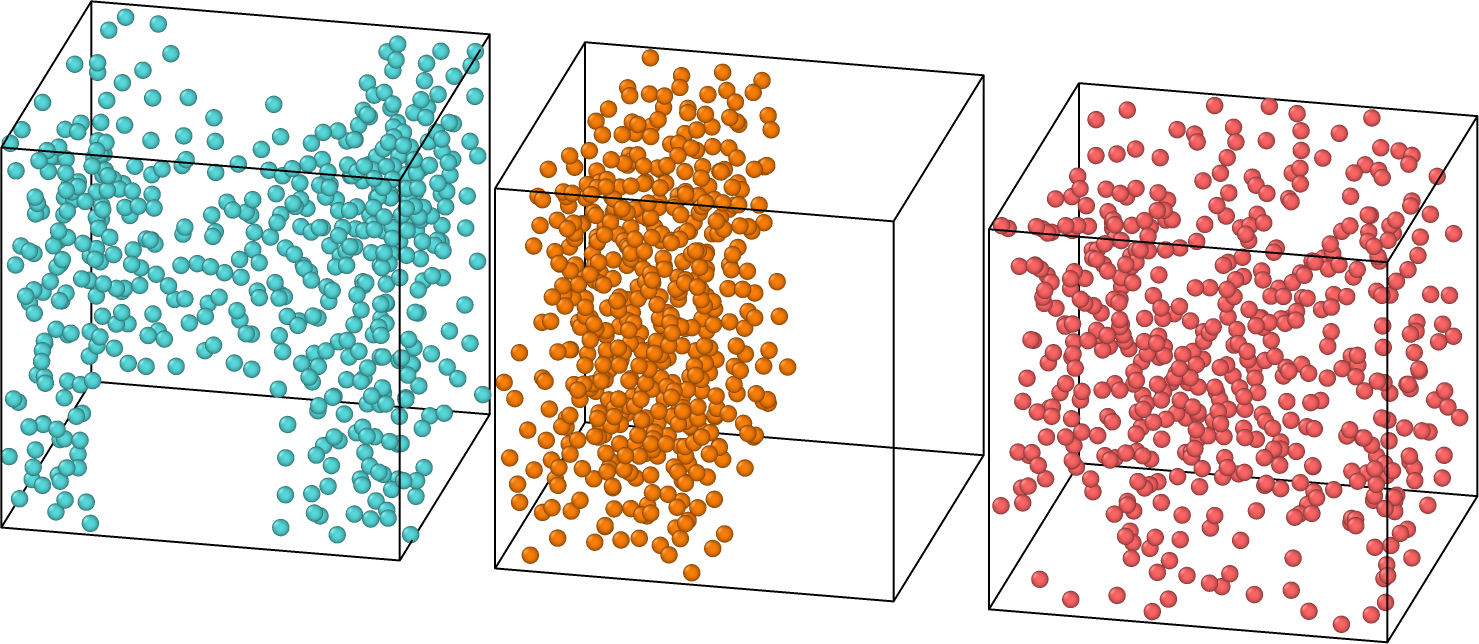
\includegraphics[width=\linewidth]{figures/Si_3_states.png}
  \caption{Three different states of Si simulated with the Stillinger-Weber potential. From the left we have Si in a solid state (blue) at $T = 400$ K, a liquid state (orange) at $T = 3000$ K and a gas state at $T = 8000$ K }
  \label{fig:3_states}
\end{figure}
On the figure we see that the solid arranges itself in a more detailed defined structure with cluster of atoms and empty space in between. The liquid also arranges itself in a cluster but not with any distinct gaps and holes. When looking at the simulation over multiple timestep we see that the atoms in the solid simulation remain fixed in its initial area while the atoms in the liquid simulation wander slowly. In the gas state wee see that the atoms is more evenly distributed in the simulation box, and when looking at multiple timesteps, we see a great mixing of the atoms as expected.
%
%%
%
\subsection*{l) Determining diffusion constant D(T) as a function of tempereture}
We now run similar simulations as in f) but with the Stillinger-Weber potential. We find the diffusion constant as a function of temperature using the mean square displacement. See script \textit{l.in} and \textit{l.py} for more info. The result is shown in figure \ref{fig:D(T)}.
\begin{figure}[H]
  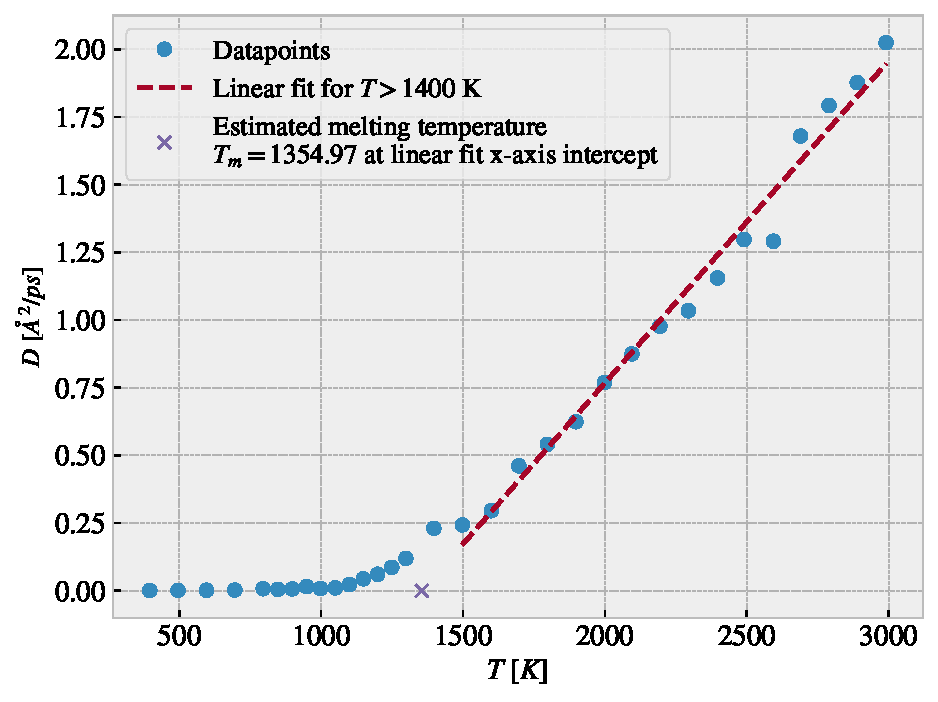
\includegraphics[width=\linewidth]{figures/D(T).pdf}
  \caption{The diffusion constant $D(T)$ as a function of temperature $T$. We se that the diffusion constant is approximately equal to zero until the estimated melting point $T_M = 1191.85$ K found as the intercept with the x-axis for a linear fit at $T > 1000$ K.}
  \label{fig:D(T)}
\end{figure}
From the development of the diffusion constant as a function of $T$ we see that there is a radical change around the esitmated melting point $T_M = 1191.85$ K. This is the point where the atoms starts to break out of the crystal structure and travel around. We didn't control the pressure which will effect the melting temperature, and this might explain the deviation from the known melting temperature at $T_{\text{melting}} = 1687 $ K and the found melting temperature $T_m = 1191.85$ K.
%
%%
%
\subsection*{m) SPCE water system}
Using the water SPCE system we calculate $D(T)$ and $g(r)$ with similar methods as used in g) and l). See script \textit{m.in} and \textit{m.py} for more info. The results are shown in figure \ref{fig:water_D} and \ref{fig:water_rdf}.
\begin{figure}[H]
  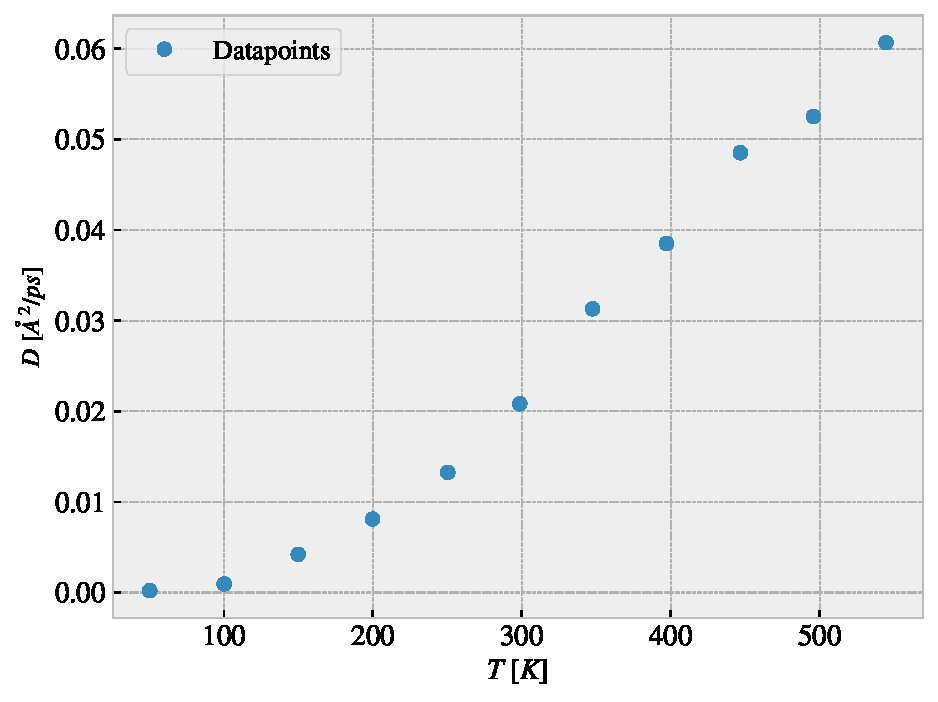
\includegraphics[width=\linewidth]{figures/water_D(T).pdf}
  \caption{Diffusion constant for water SPCE as a function of temperature}
  \label{fig:water_D}
\end{figure}
\begin{figure}[H]
  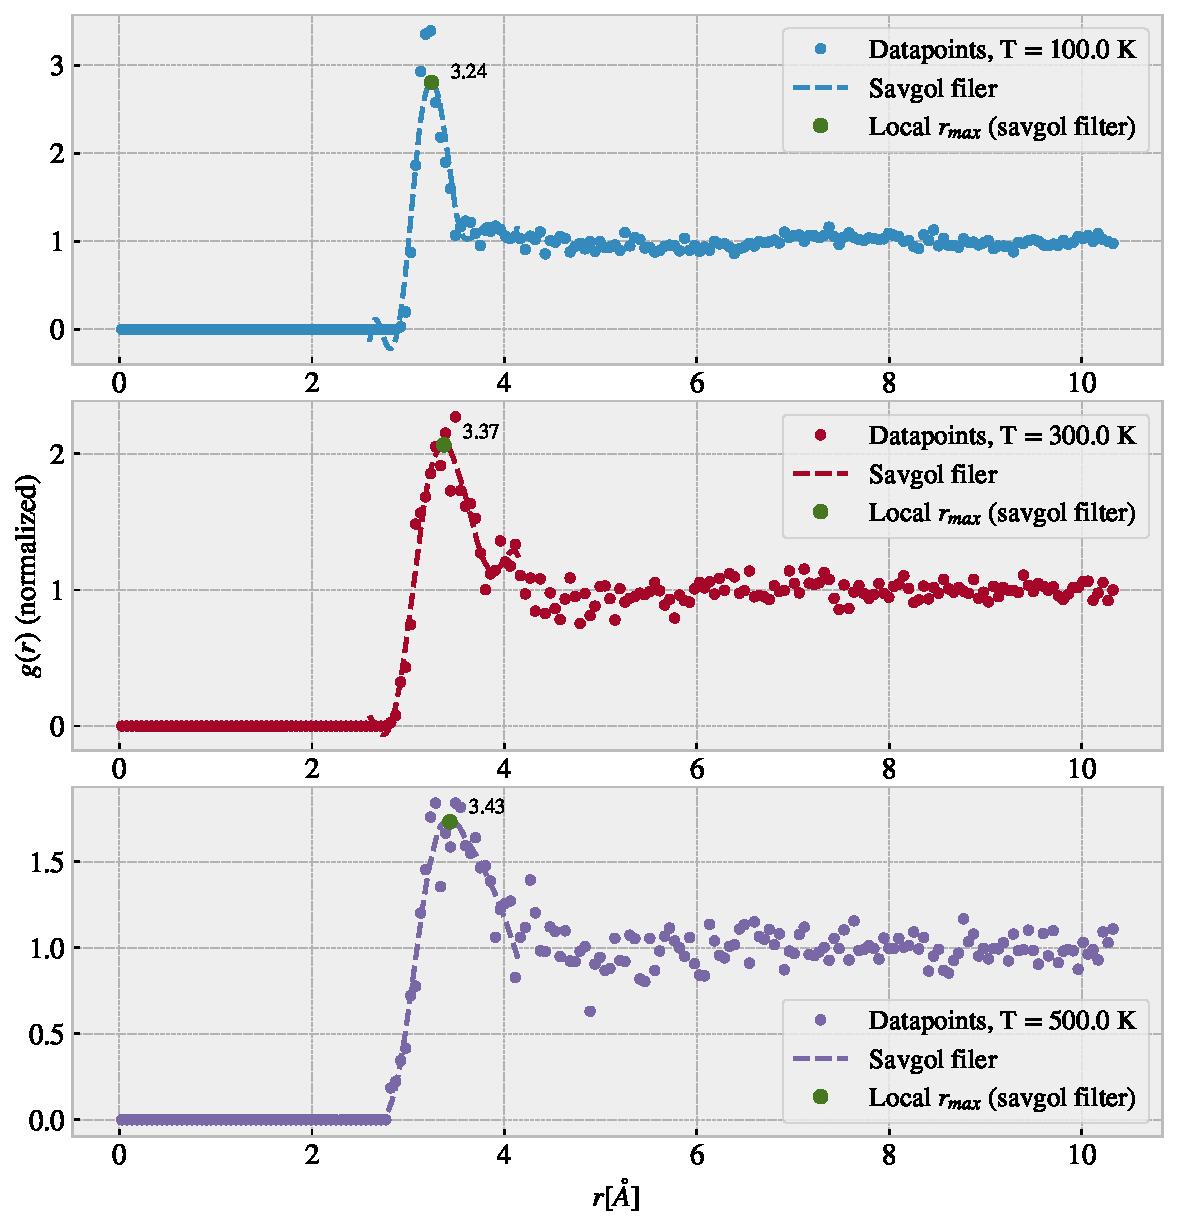
\includegraphics[width=\linewidth]{figures/water_rdf.pdf}
  \caption{Radial distribution for water with SPCE for three different temperatures correpsonding to expected solid, liquid and gas phase. }
  \label{fig:water_rdf}
\end{figure}

From figure \ref{fig:water_D} we see a somewhat linear trend similar to the result for liquid argon (figure \ref{fig:diffusion_relation}) and melted Si (figure \ref{fig:D(T)}). We would expect $D(T) = 0$ at the melting temperature of water at $273.14 (100 ^{\circ})$. This is not the case here, and this tell us that the low temperature behaviour isn't very accurate. When looking at the radial distribution in figure \ref{fig:water_rdf} we see almost no difference between the temperatures 100 K, 300 K and 500 K, which should represent all the three phases of solid, liquid and gas. From this we must conclude that the model (under our simulation conditions) lack the ability to describe the phase transistions. However it seem to work great as a description of the material transport (diffusion) as a function of temperature at higher temperatures.


\bibliographystyle{unsrt}
\bibliography{Bibliography.bib}





\end{document}
